In order to evaluate the correctness of our parallel algorithm, we
produced a real-time 3D visualization of the simulation's output data
using R. The simulation generates its own input (the initial locations
and headings of each bird) and provides several configuration
options. By default, each bird is positioned randomly throughout the
universe. In addition we provide functionality for modeling distinct
clusters of birds in order to simulate interactions between flocks.
The simulation output is a .csv file which contains all bird positions
over each time-step. Using this output, we can plot the flock at each
time-step, and compile these plots into a video for visualization. All
of this is accomplished automatically in a run script.

\begin{figure}[h!]
  \centering
  \begin{subfigure}{0.24\textwidth}
    \centering
    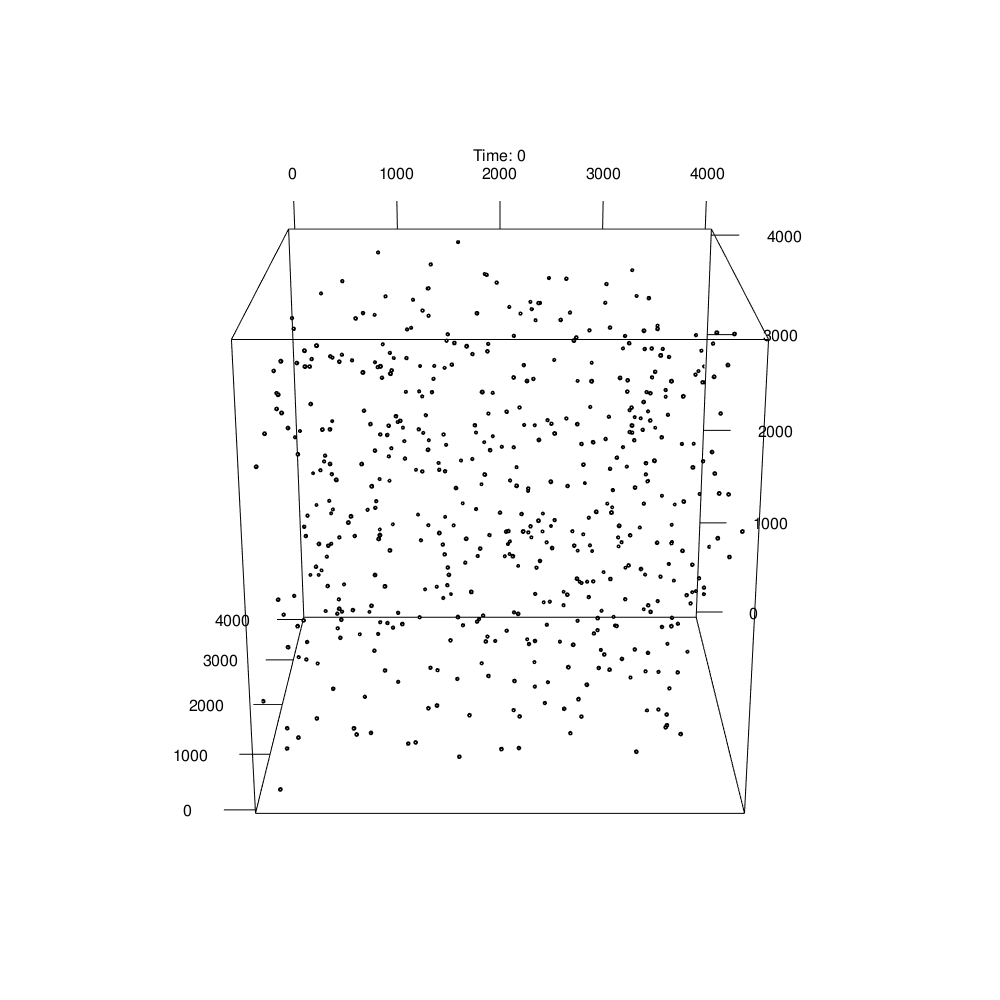
\includegraphics[width=\textwidth]{fig1-0000.png}
    \caption{Time = 0}
  \end{subfigure}
  \begin{subfigure}{0.24\textwidth}
    \centering
    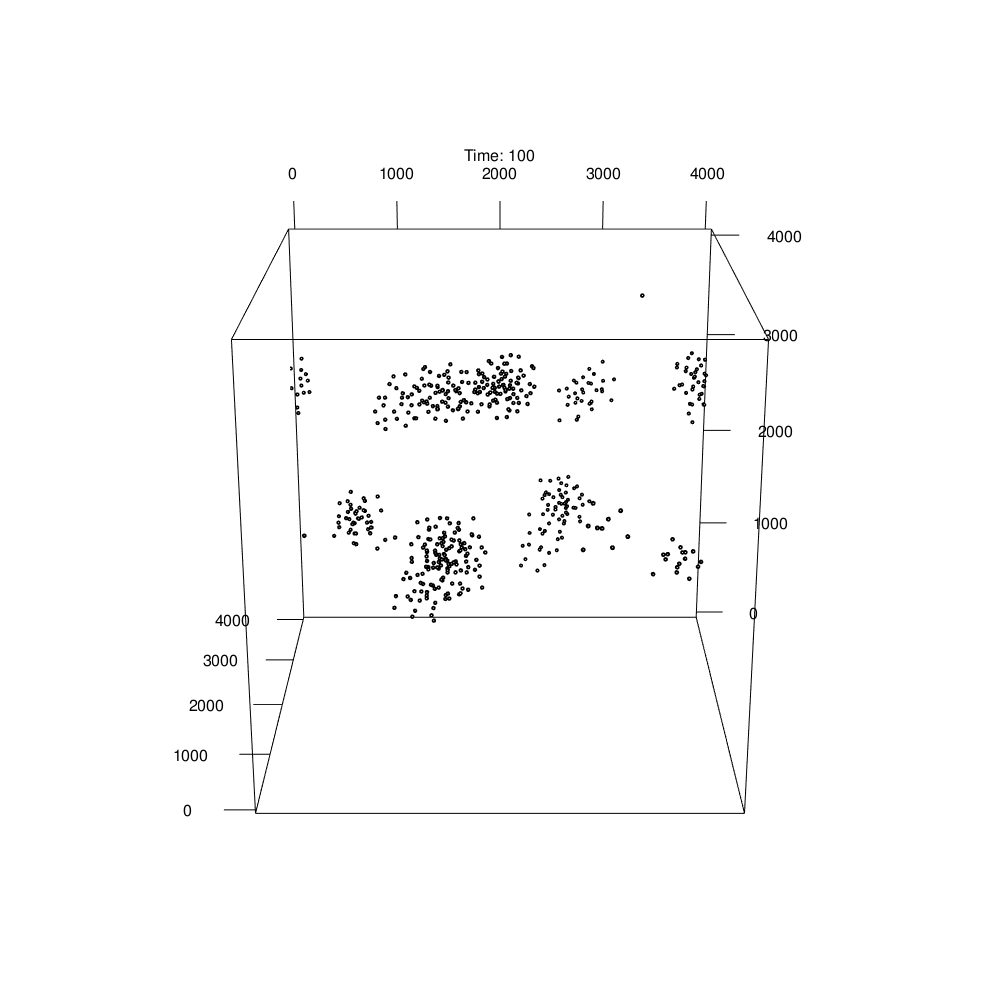
\includegraphics[width=\textwidth]{fig1-0100.png}
    \caption{Time = 100}
  \end{subfigure}
  \begin{subfigure}{0.24\textwidth}
    \centering
    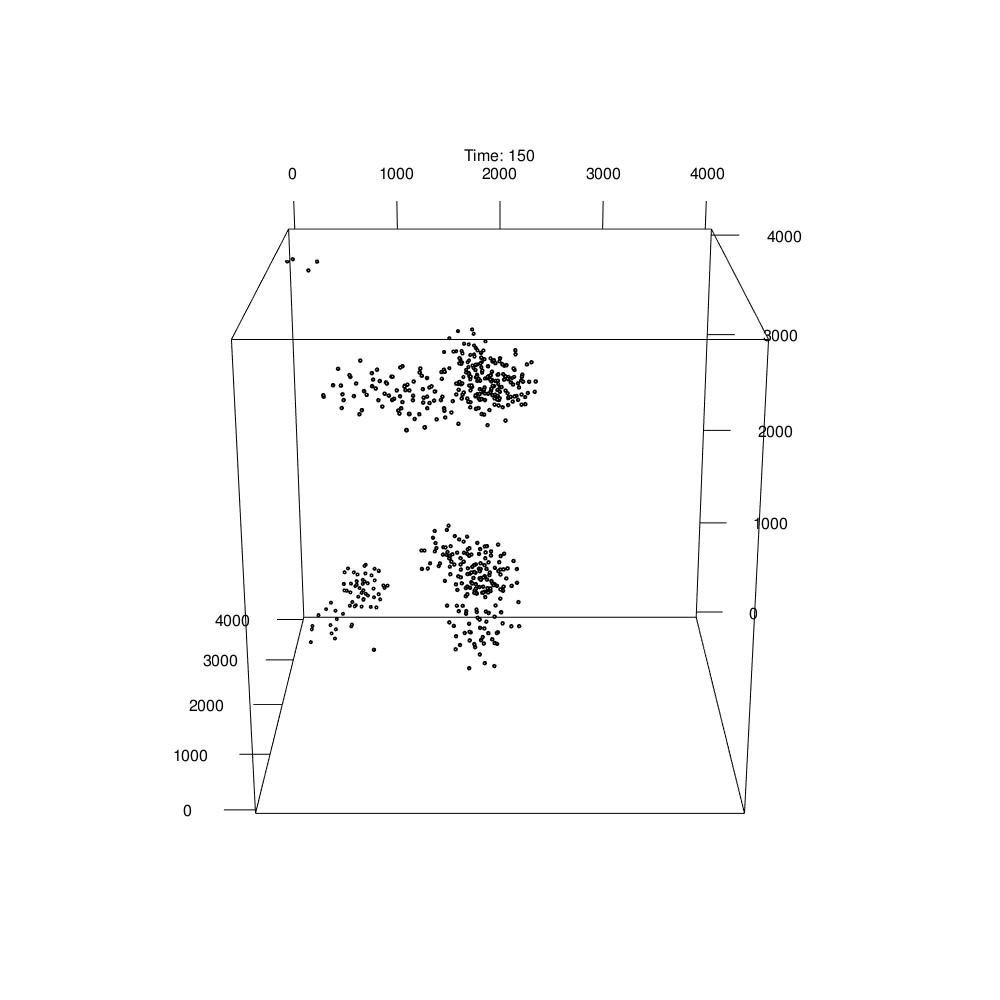
\includegraphics[width=\textwidth]{fig1-0150.png}
    \caption{Time = 150}
  \end{subfigure}
  \begin{subfigure}{0.24\textwidth}
    \centering
    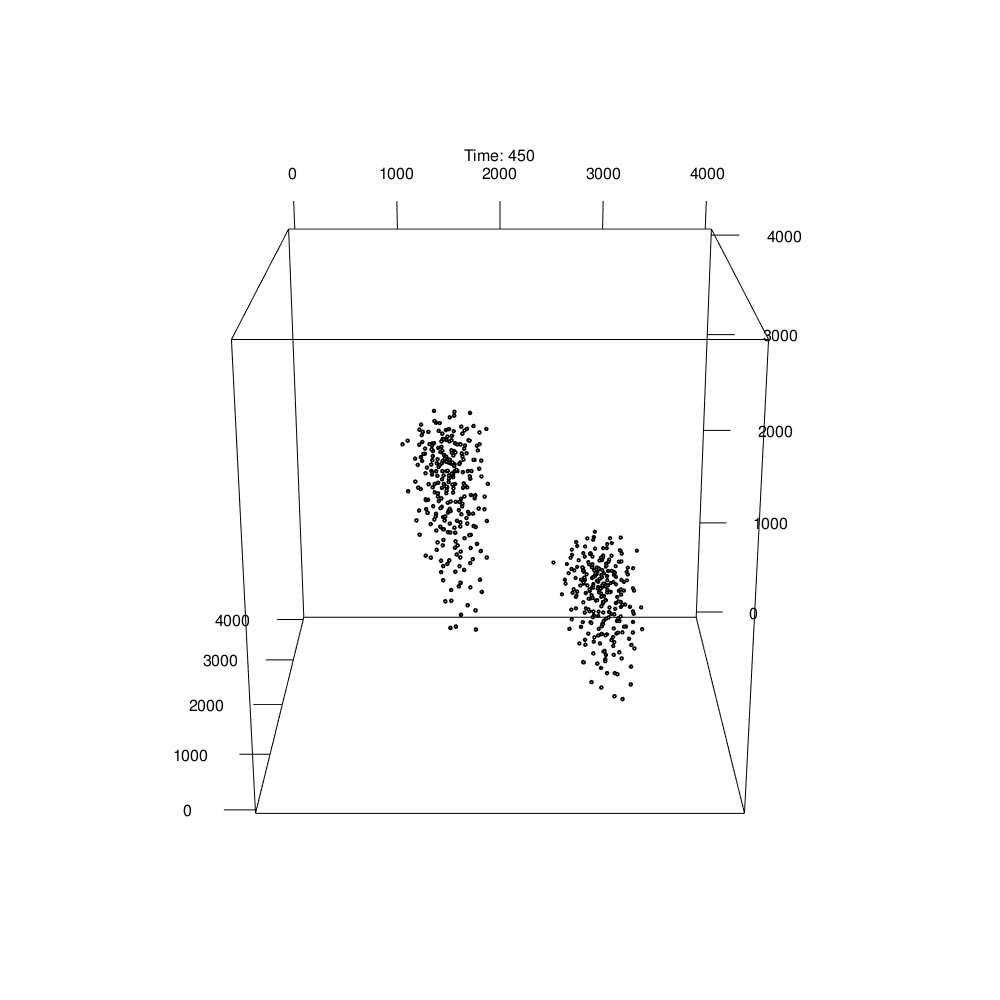
\includegraphics[width=\textwidth]{fig1-0450.png}
    \caption{Time = 450}
  \end{subfigure}
  
  \caption{Simulation visualizations with random initialization after
    0, 100, 150, and 450 time-steps}
  \label{fig:visuals}
\end{figure}

Figure \ref{fig:visuals} displays plots of a randomly initialized
flock of birds after 0, 100, 150, and 450 time-steps. At simulation
time 0, there is no pattern guiding the birds. But already after 100
iterations, we find that distinct flocks are beginning to emerge. At
time-step 150, there are roughly three flocks of birds within the
universe, and by time-step 450, they have merged into two uniform
flocks. Thus we find that there is little need for cluster
initialization, since over time even randomly positioned birds
gradually and naturally form these clusters. This result is not only
fascinating from a biological and cognitive perspective, but also is
a testament to the accuracy of the simulation--- over time, we find
that these simple rules generate flocks which behave in a manner
remarkably similar to real flocks of birds.

Interestingly enough, these rules can also be used to produce emergent
divergence of flocks which are too large. In order to accomplish this,
we ran a simulation of 8192 birds separated into two flocks in a
universe of size 10000. Since each flock was substantially larger than
the neighbor radius of the individual birds, alignment and cohesion
had little effect. Instead, the crowding of birds within these larger
flocks caused the separation rule to gradually pull the flocks apart,
creating a larger number of more spacious flocks.

\begin{figure}[h!]
  \centering
  \begin{subfigure}{0.24\textwidth}
    \centering
    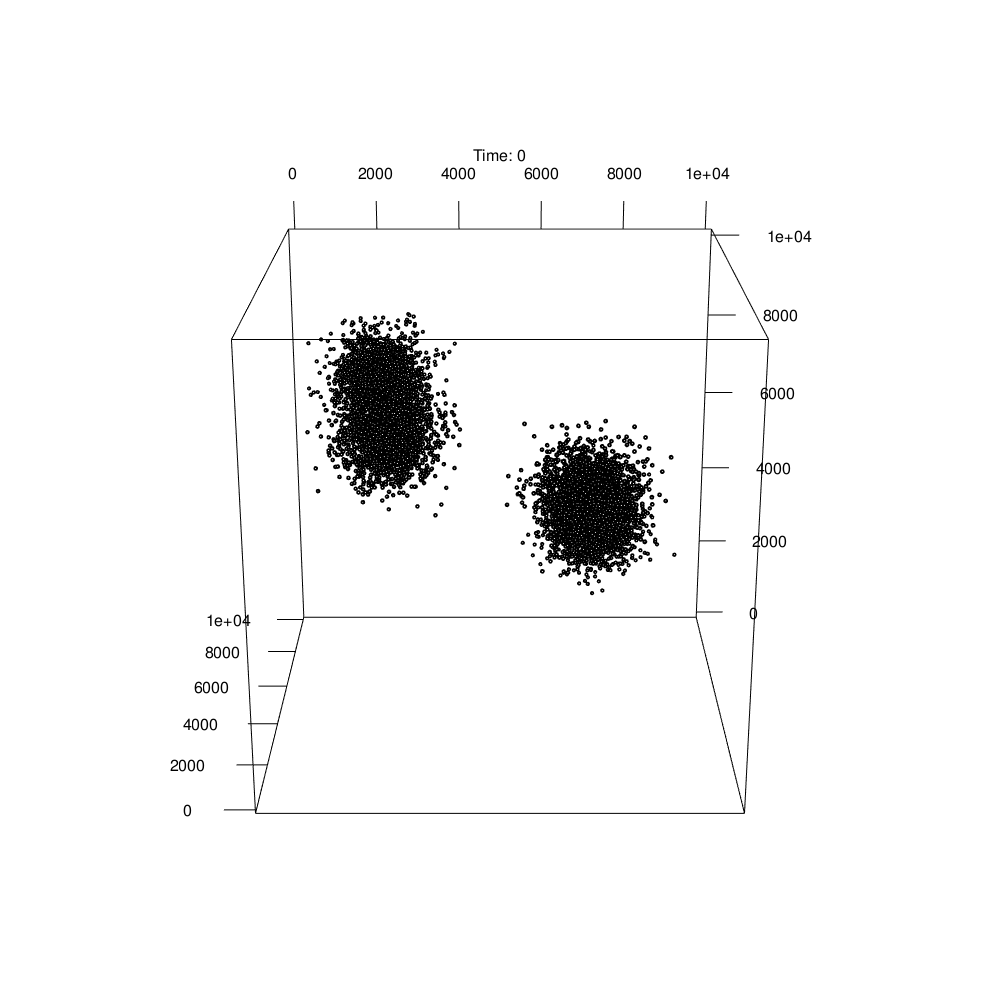
\includegraphics[width=\textwidth]{fig2-00.png}
    \caption{Time = 0}
  \end{subfigure}
  \begin{subfigure}{0.24\textwidth}
    \centering
    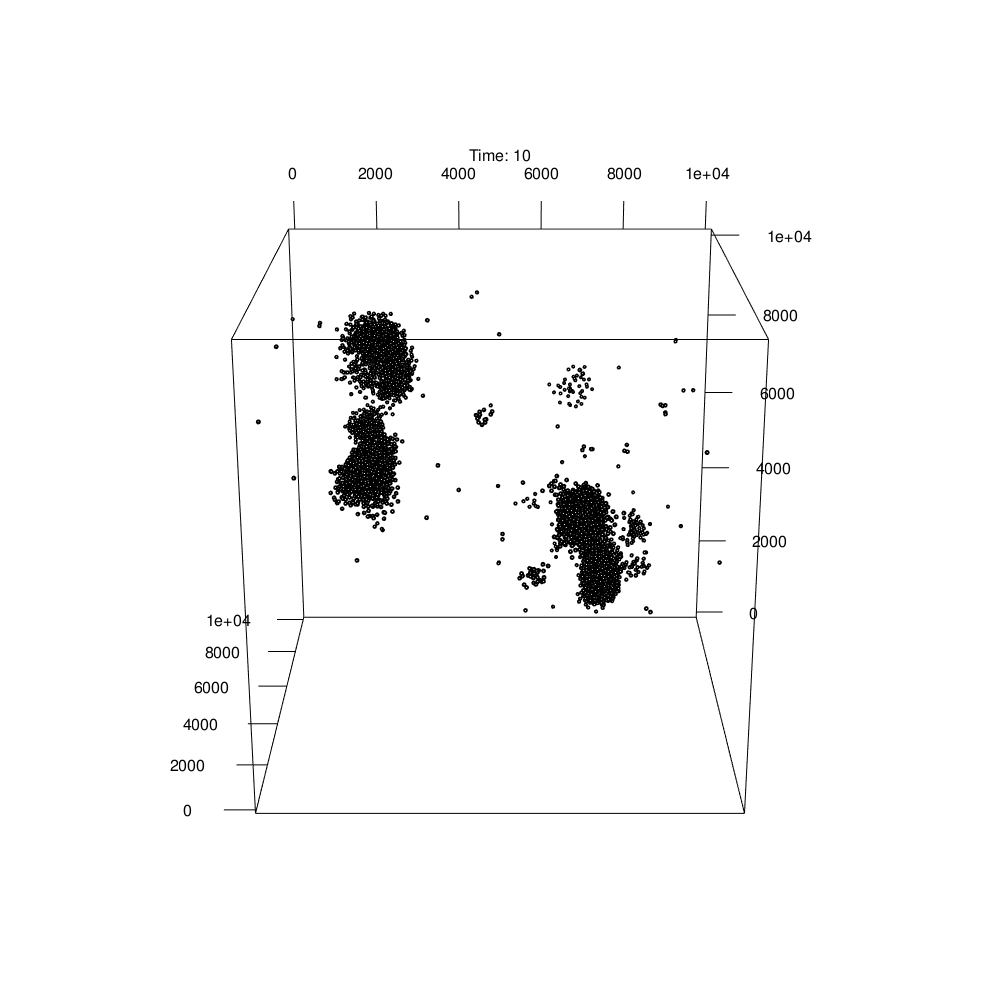
\includegraphics[width=\textwidth]{fig2-10.png}
    \caption{Time = 10}
  \end{subfigure}
  \begin{subfigure}{0.24\textwidth}
    \centering
    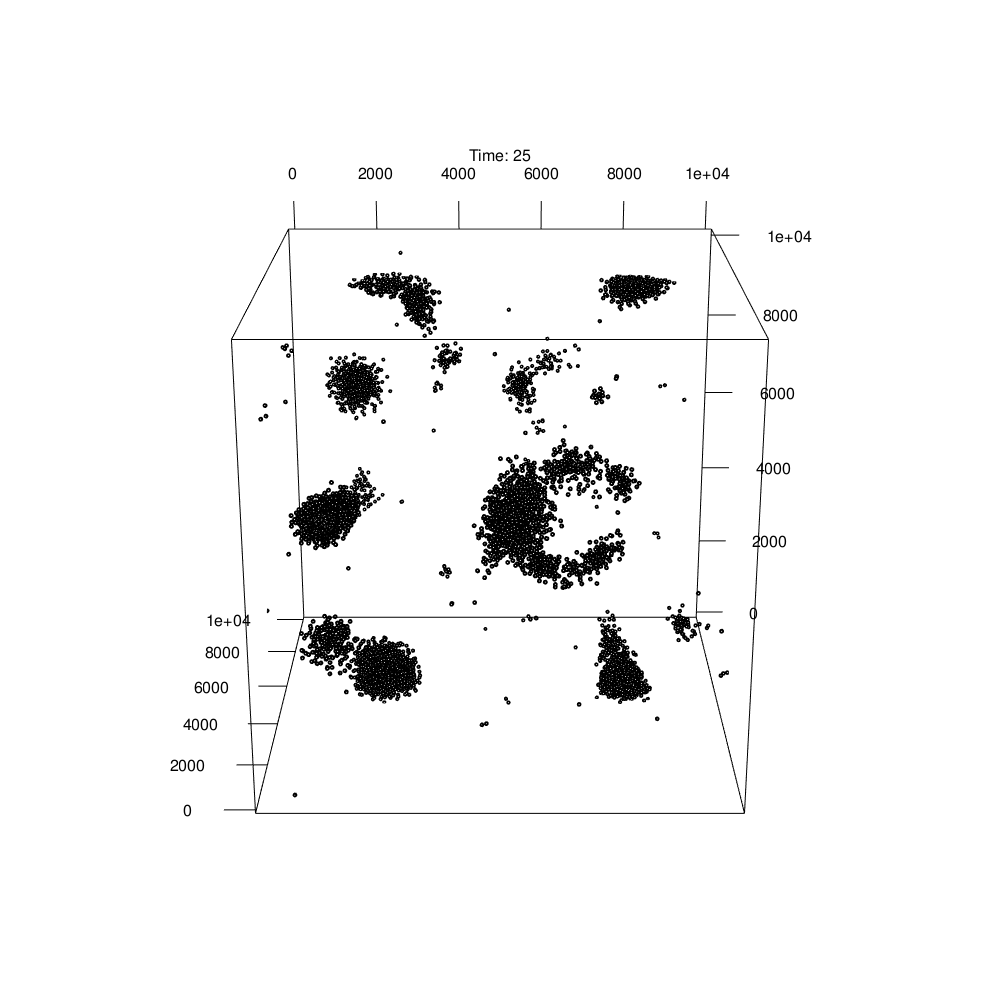
\includegraphics[width=\textwidth]{fig2-25.png}
    \caption{Time = 25}
  \end{subfigure}
  \begin{subfigure}{0.24\textwidth}
    \centering
    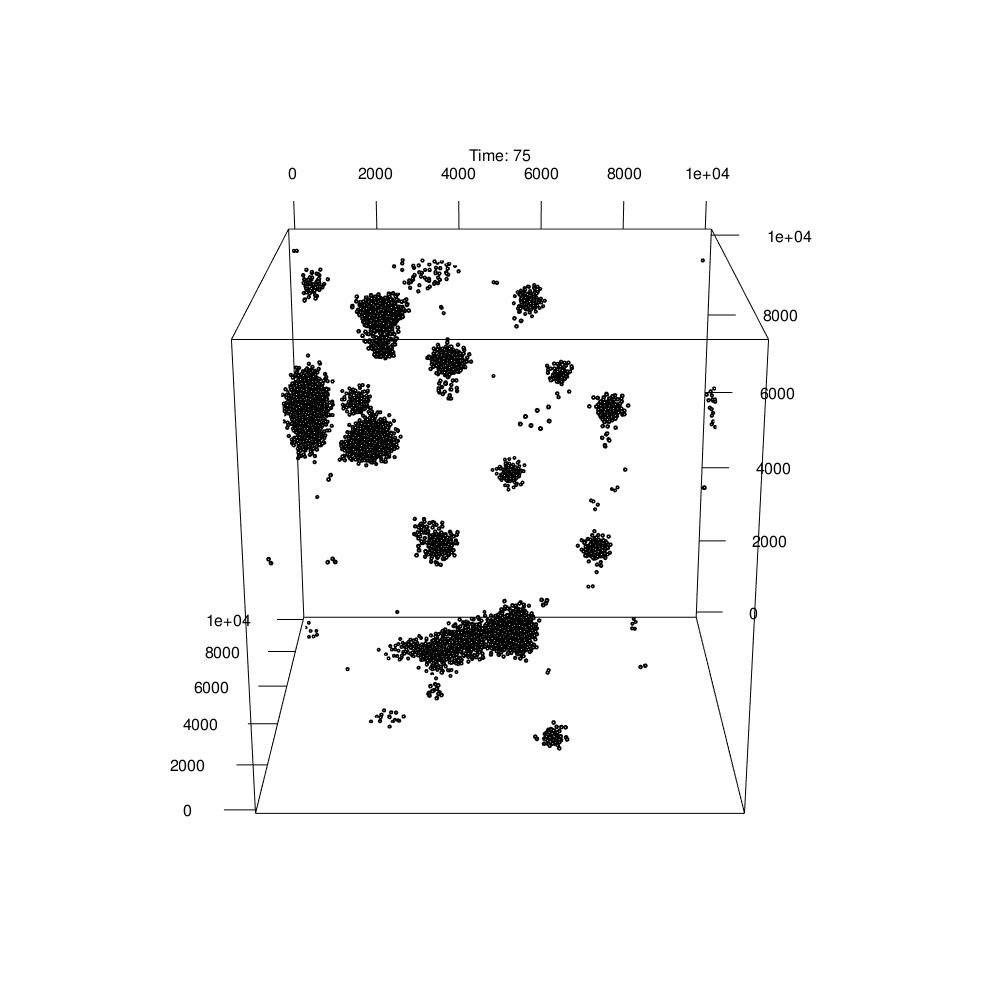
\includegraphics[width=\textwidth]{fig2-75.png}
    \caption{Time = 75}
  \end{subfigure}
  
  \caption{Simulation visualizations with cluster initialization after
    0, 10, 25, and 75 time-steps}
  \label{fig:visuals}
\end{figure}

The visualization software was originally implemented in R in two
dimensions by Mitchell Mellone, then modified for three dimensions by
Kevin O'Neill.
